\chapter{Perancangan}

\section{Perancangan Antarmuka}
Perangkat lunak yang dibangun akan menggunakan tampilan antarmuka grafis. Tampilan antarmuka ini digunakan agar mempermudah interaksi pengguna dengan perangkat lunak. Selain itu, jenis tampilan ini juga digunakan untuk menghasilkan visualisasi penempatan kamera CCTV sehingga pengguna dapat memahami penempatan-penempatan tersebut secara visual. Pada bagian ini akan dijelaskan bentuk dari setiap antarmuka yang terdapat dalam perangkat lunak. Berikut bentuk antarmuka tersebut:

\begin{itemize}
	\item Antarmuka: \textbf{Penerima Masukan}\\
	Antarmuka ini berfungsi untuk menerima masukan dari pengguna seperti pada gambar~\ref{fig:input_mockup}. Pada antarmuka ini terdapat kolom-kolom masukan yang dapat diisi oleh pengguna. Pengguna dapat mengisi ukuran ruangan, spesifikasi kamera CCTV, ukuran terbesar cell, dan jumlah kemungkinan arah pandang kamera CCTV pada kolom tersebut. Apabila pengguna sudah yakin dengan masukan yang diberikan, maka pengguna dapat menekan tombol ''\textit{submit}'' yang akan mengarahkan pengguna pada antarmuka penempatan kamera CCTV.

	\begin{figure}[h]
		\centering  
		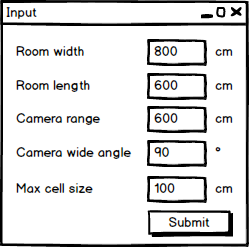
\includegraphics[scale=0.6]{input_mockup}
		\caption[Perancangan antarmuka penerima masukan]{Perancangan antarmuka penerima masukan}
		\label{fig:input_mockup}
	\end{figure}

	\item Antarmuka: \textbf{Penempatan Kamera CCTV}\\
	Antarmuka ini berfungsi untuk menampilkan solusi masalah penempatan kamera CCTV yang berjumlah minimum yang dapat mencakup seluruh isi ruangan seperti pada gambar~\ref{fig:simulator_mockup}. Di dalam antarmuka ini terdapat 2 bagian, yaitu:
	\begin{itemize}
		\item Panel informasi\\
		Panel ini berada di bagian kiri antarmuka yang berfungsi untuk memberikan informasi mengenai spesifikasi masalah dan solusi masalah. Solusi masalah yang terdiri dari penempatan-penempatan kamera CCTV dapat dilihat pada bagian daftar kamera CCTV (\textit{Camera List}). Pada setiap baris penempatan terdapat informasi titik lokasi penempatan dan juga sudut arah pandang yang dituju.
		
		\item Panel visualisasi penempatan kamera CCTV\\
		Panel ini berada di bagian kanan antarmuka yang berfungsi untuk menampilkan visualisasi matriks \textit{cell} dan penempatan kamera CCTV.
	\end{itemize}
	\begin{figure}[h]
		\centering  
		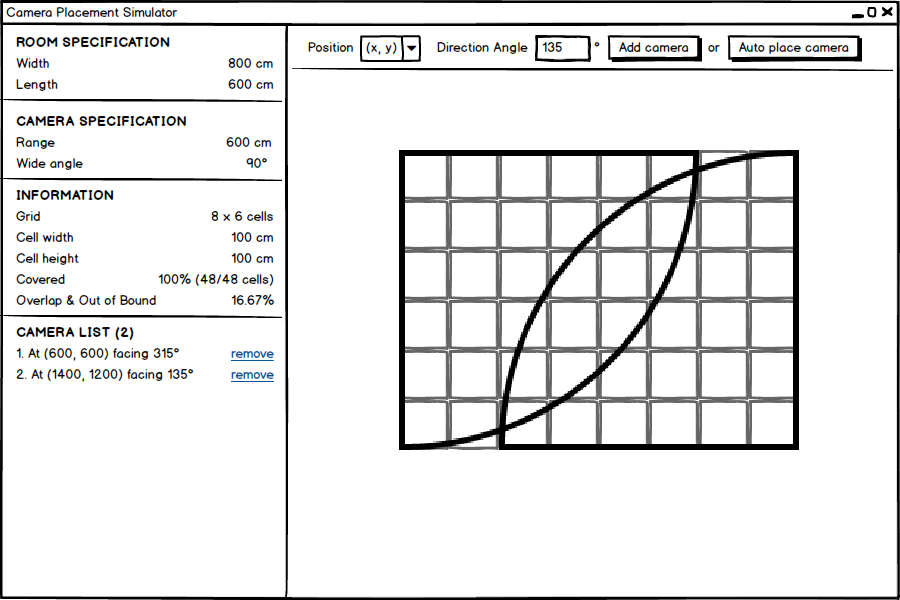
\includegraphics[scale=0.4]{simulator_mockup}
		\caption[Perancangan antarmuka penempatan kamera CCTV]{Perancangan antarmuka penempatan kamera CCTV}
		\label{fig:simulator_mockup}
	\end{figure}
\end{itemize}

\section{Perancangan Kelas}
Rancangan awal kelas-kelas yang telah dipaparkan di~\ref{subsec:diagram_kelas_sederhana} akan dikembangkan lebih lanjut. Kelas-kelas yang digunakan untuk memodelkan masalah diletakkan dalam \textit{package} model. Kelas-kelas untuk memodelkan dan menyelesaikan masalah \textit{binary integer programming} diletakkan pada \textit{package} bip. Diagram kelas rinci untuk kedua package tersebut dapat dilihat pada gambar~\ref{fig:class_diagram_model_complete} dan~\ref{fig:class_diagram_bip_complete}.

\begin{sidewaysfigure}
	\centering  
	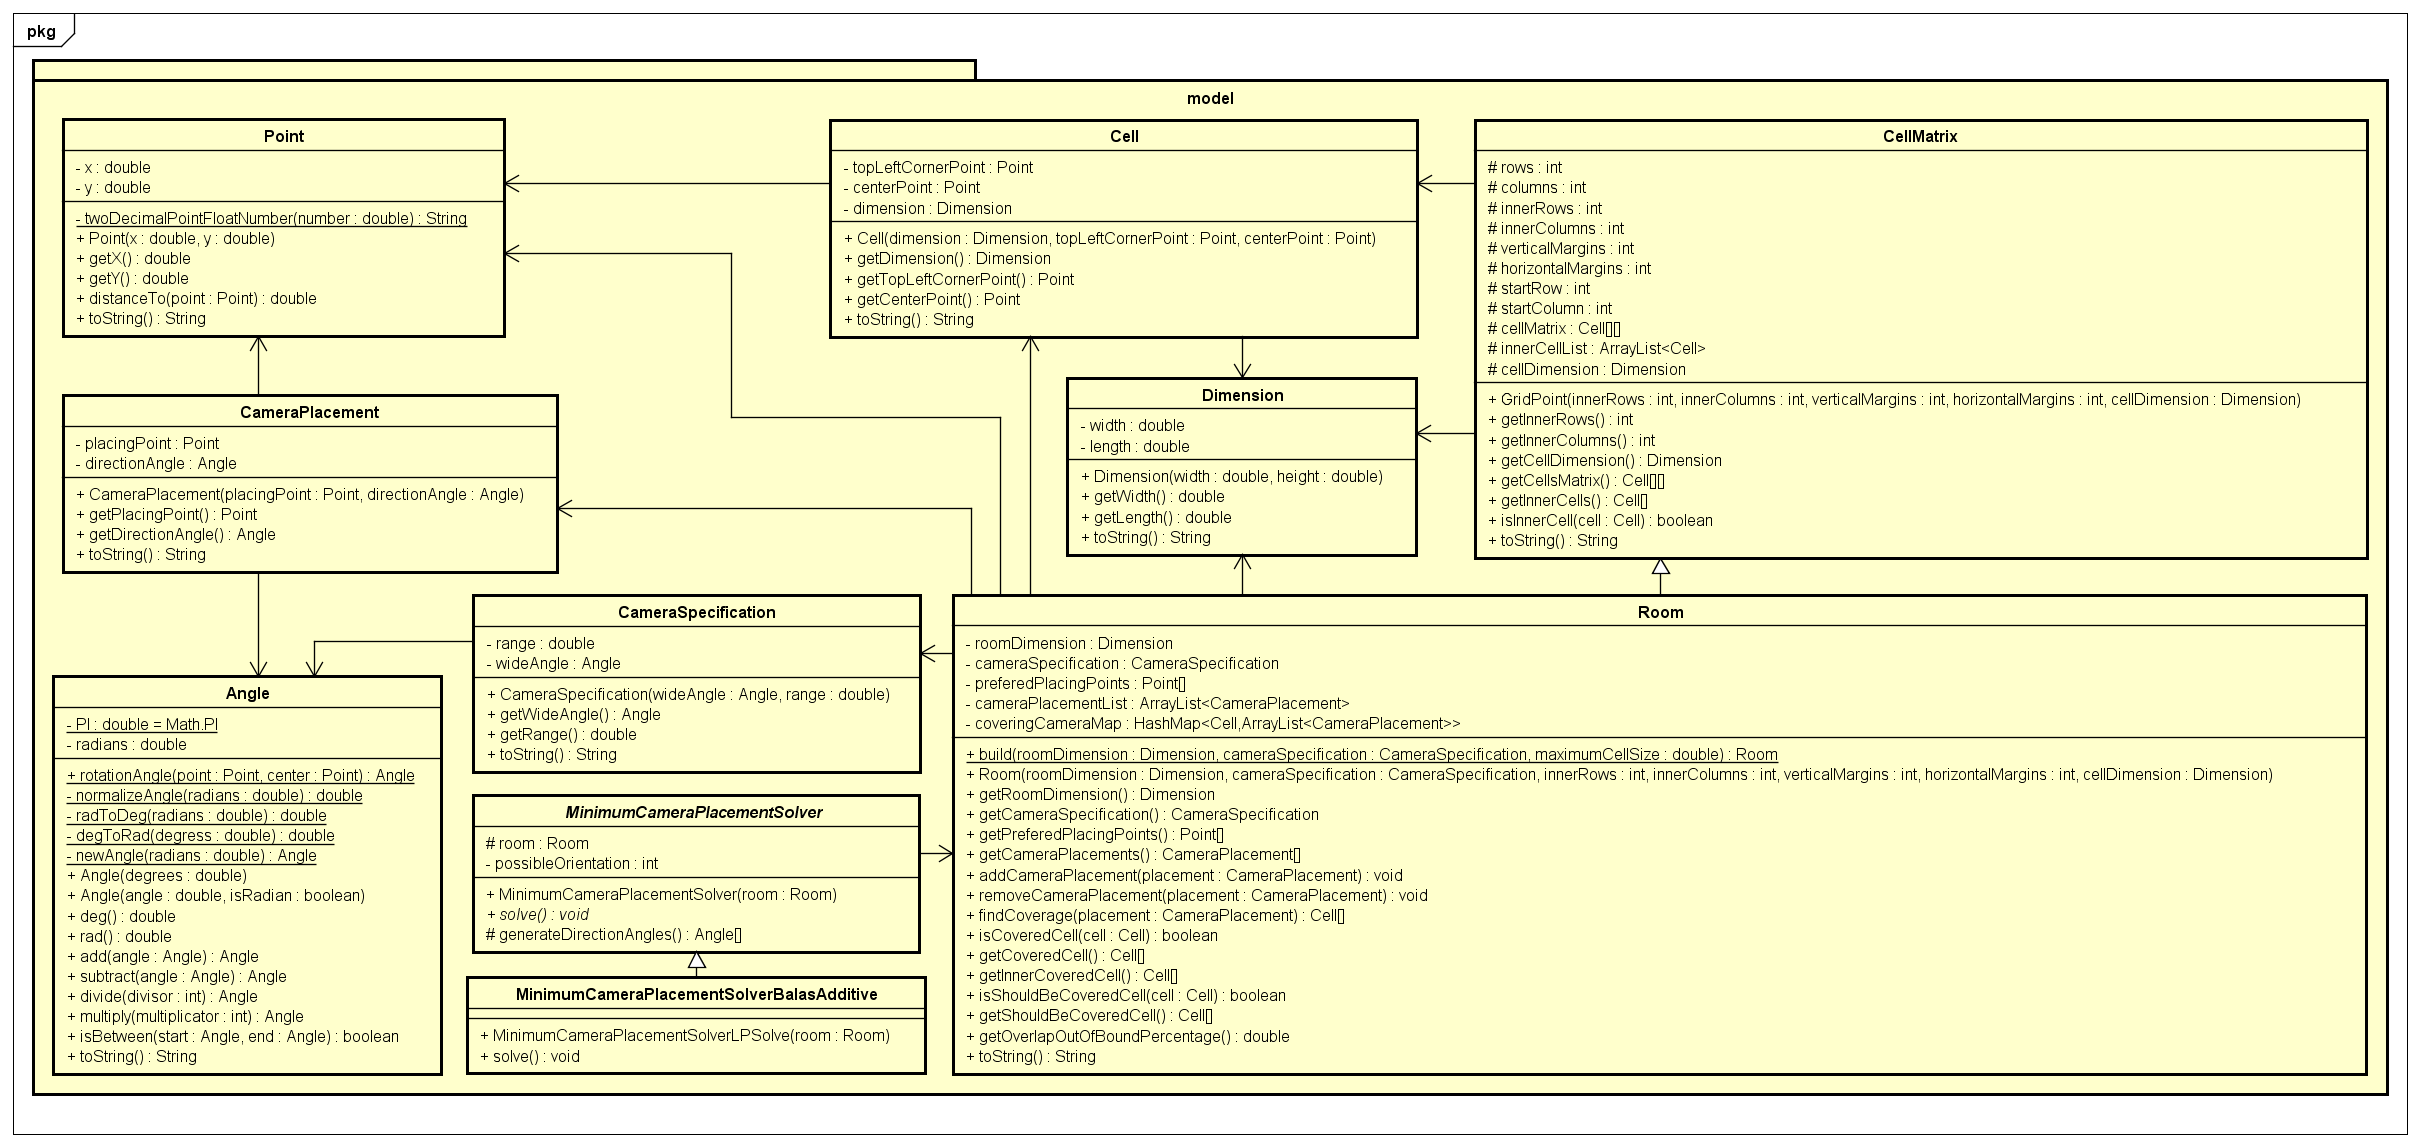
\includegraphics[scale=0.38]{class_diagram_model_complete}
	\caption[Diagram kelas rinci untuk \textit{package} model]{Diagram kelas rinci untuk \textit{package} model}
	\label{fig:class_diagram_model_complete}
\end{sidewaysfigure}

\begin{sidewaysfigure}
	\centering  
	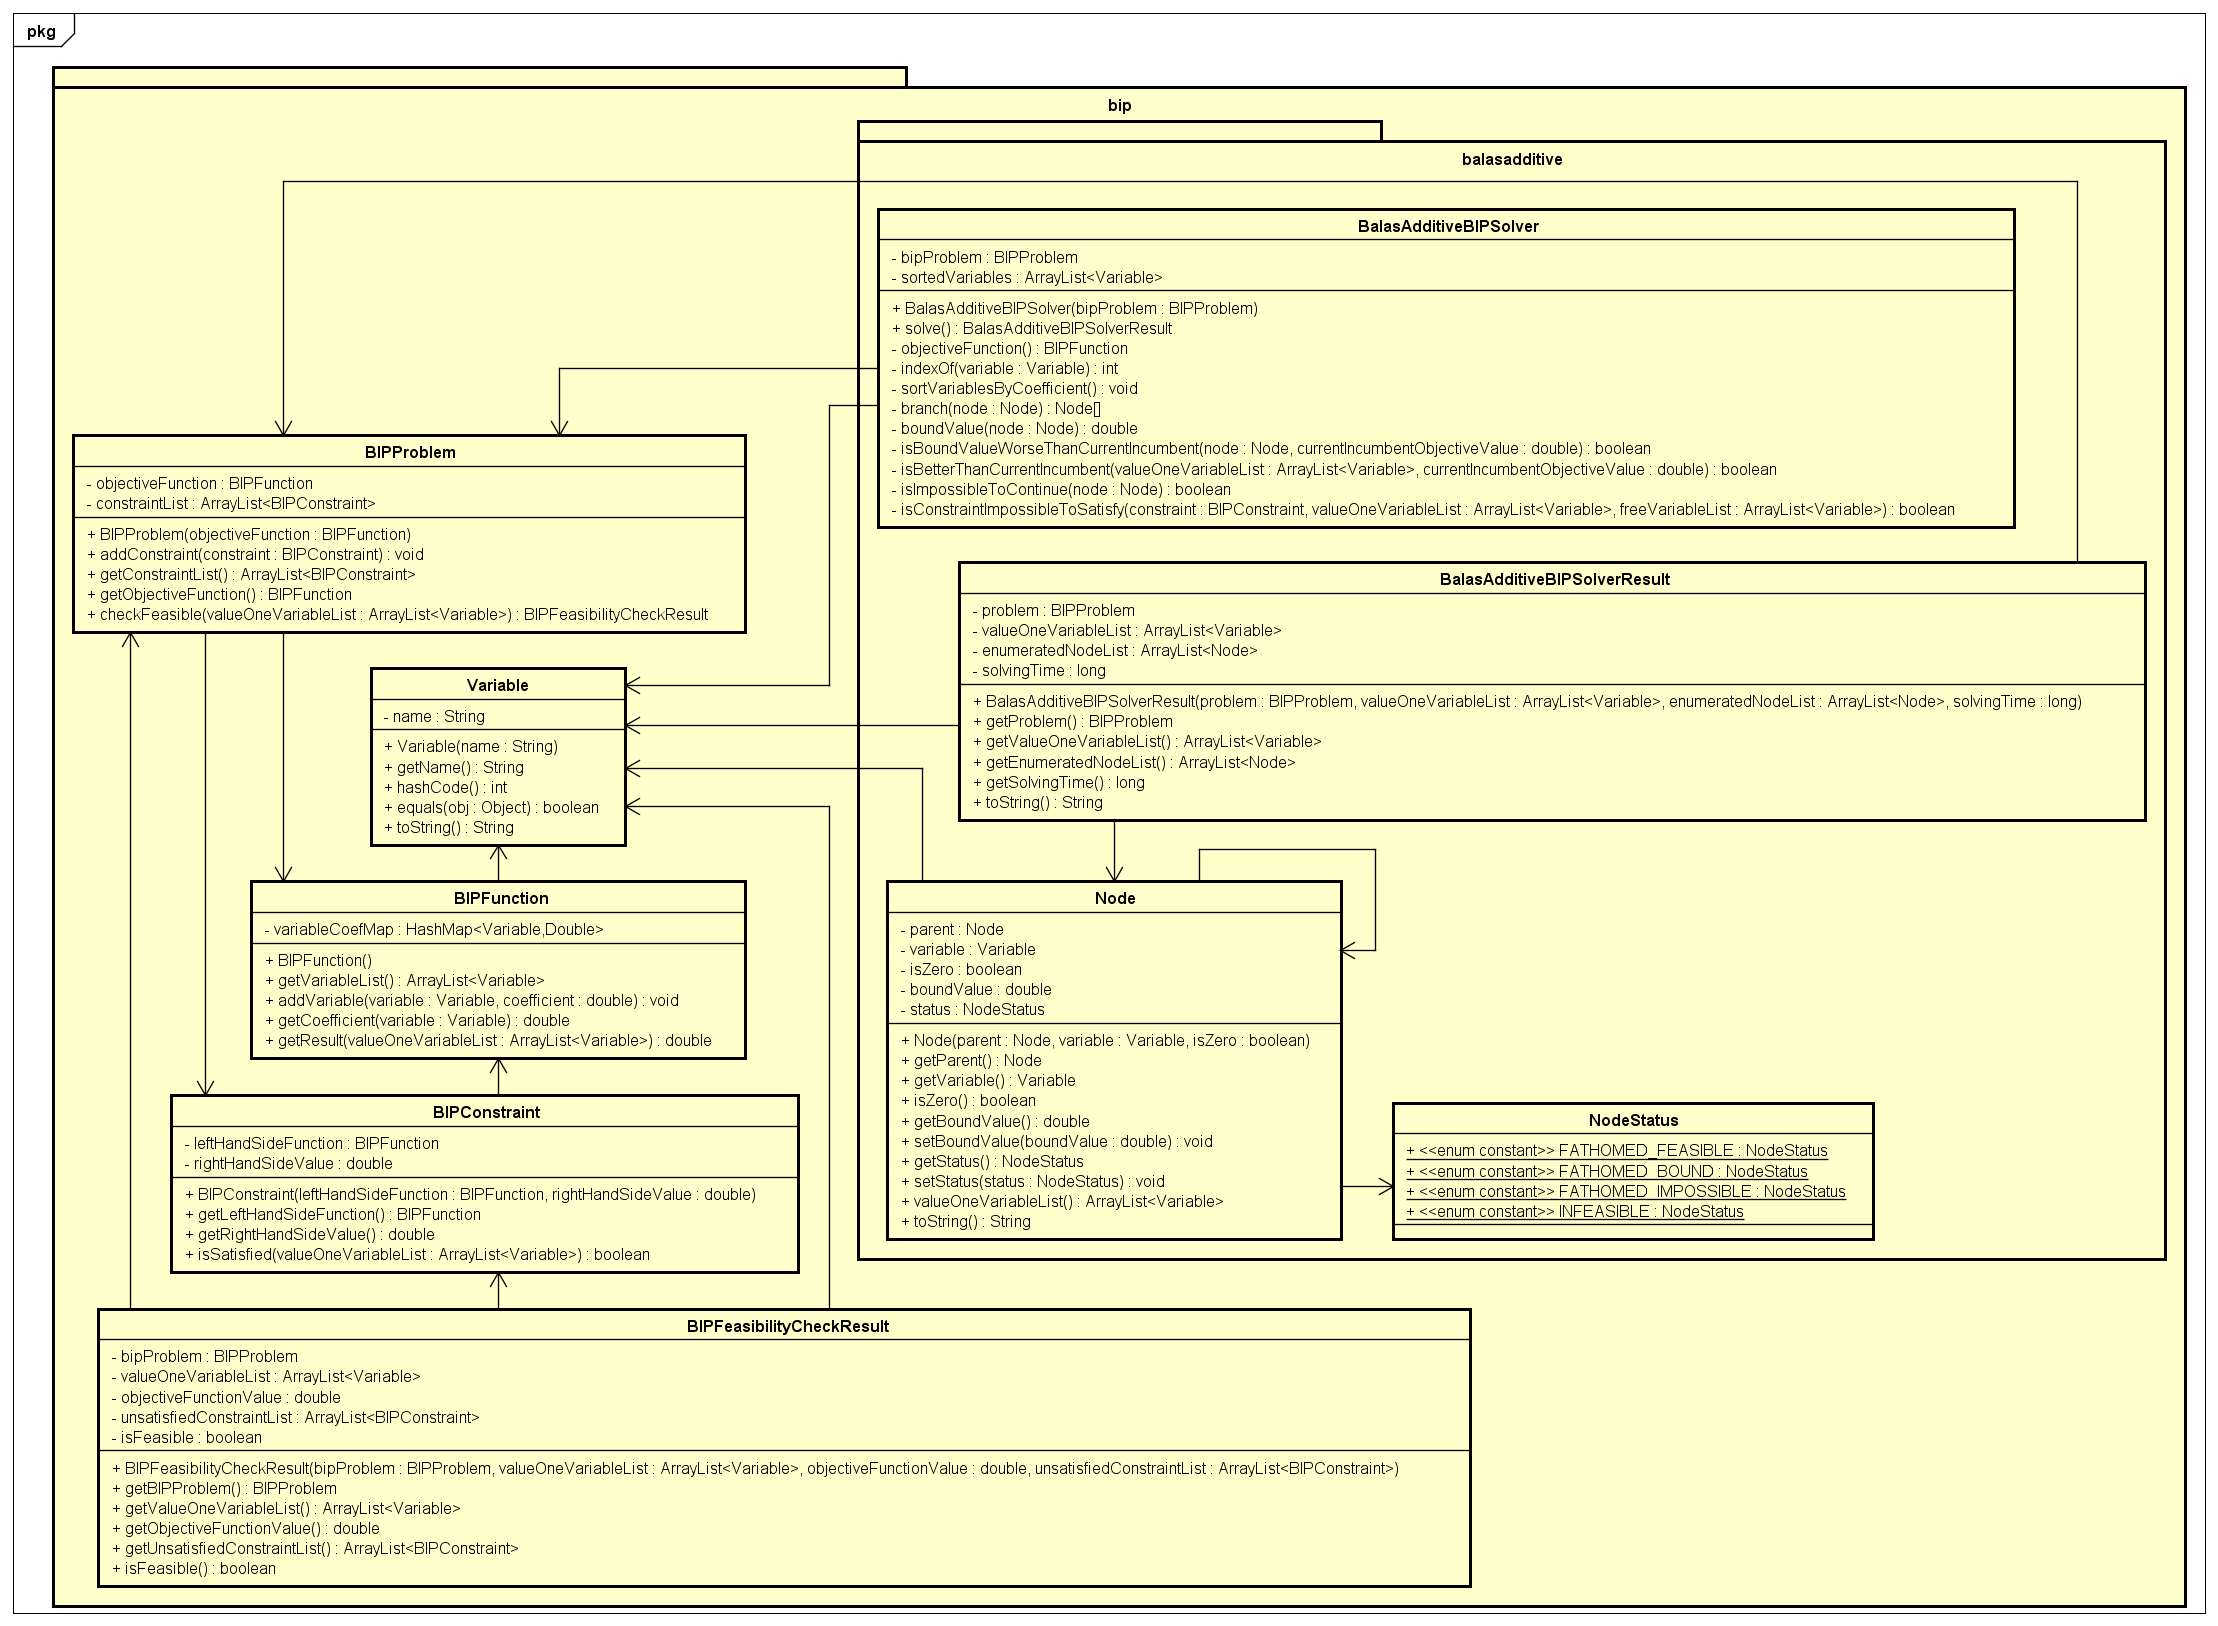
\includegraphics[scale=0.33]{class_diagram_bip_complete}
	\caption[Diagram kelas rinci untuk \textit{package} bip dan \textit{subpackage} balasadditive]{Diagram kelas rinci untuk \textit{package} bip dan \textit{subpackage} balasadditive}
	\label{fig:class_diagram_bip_complete}
\end{sidewaysfigure}

\subsection{Kelas \textit{Angle}}
\begin{figure}[H]
	\centering  
	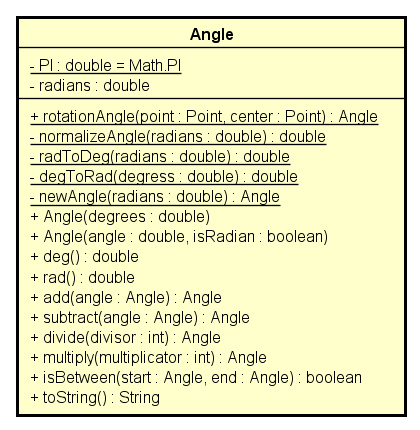
\includegraphics[scale=0.6]{class_angle}
	\caption[Diagram kelas \textit{Angle}]{Diagram kelas \textit{Angle}}
	\label{fig:class_angle}
\end{figure}
	
Kelas ini merepresentasikan sudut dan menangani fungsi-fungsi yang berhubungan dengan sudut. Diagram kelas \textit{Angle} dapat dilihat pada gambar~\ref{fig:class_angle}. Berikut ini merupakan atribut-atribut yang terdapat pada kelas \textit{Angle}:
\begin{itemize}
	\item \textbf{\textit{PI} \(\rightarrow\) \textit{double}}\\
	Atribut ini merupakan atribut statis bernilai \(\pi\) yang dapat digunakan oleh setiap objek dari kelas \textit{Angle}.
	\item \textbf{\textit{radians} \(\rightarrow\) \textit{double}}\\
	Atribut ini berguna untuk menampung sudut dalam bentuk radian.
\end{itemize}
Berikut ini merupakan fungsi-fungsi yang terdapat pada kelas \textit{Angle}:
\begin{itemize}
	\item \textbf{\textit{rotationAngle}(\textit{point} \(\rightarrow\) \textit{Point}, \textit{center} \(\rightarrow\) \textit{Point}) \(\rightarrow\) \textit{Angle}}\\
	Fungsi ini merupakan fungsi statis yang berguna untuk mendapatkan sudut rotasi dari titik \textit{point} terhadap titik \textit{center}.
	\item \textbf{\textit{normalizeAngle}(\textit{radians} \(\rightarrow\) \textit{double}) \(\rightarrow\) \textit{double}}\\
	Fungsi ini merupakan fungsi statis yang berguna untuk melakukan normalisasi sudut \textit{radians} sehingga berada dalam rentang \(0\leq\textit{radians}<2\pi\).
	\item \textbf{\textit{radToDeg}(\textit{radians} \(\rightarrow\) \textit{double}) \(\rightarrow\) \textit{double}}\\
	Fungsi ini merupakan fungsi statis yang berguna untuk mengubah sudut dalam bentuk radian menjadi sudut dalam bentuk derajat.
	\item \textbf{\textit{degToRad}(\textit{degrees} \(\rightarrow\) \textit{double}) \(\rightarrow\) \textit{double}}\\
	Fungsi ini merupakan fungsi statis yang berguna untuk mengubah sudut dalam bentuk derajat menjadi sudut dalam bentuk radian.
	\item \textbf{\textit{newAngle}(\textit{radians} \(\rightarrow\) \textit{double}) \(\rightarrow\) \textit{Angle}}\\
	Fungsi ini merupakan fungsi statis yang berguna untuk membuat objek \textit{Angle} baru.
	\item \textbf{\textit{deg}() \(\rightarrow\) \textit{double}}\\
	Fungsi ini berguna untuk mendapatkan sudut dalam bentuk derajat.
	\item \textbf{\textit{rad}() \(\rightarrow\) \textit{double}}\\
	Fungsi ini berguna untuk mendapatkan sudut dalam bentuk radian.
	\item \textbf{\textit{add}(\textit{angle} \(\rightarrow\) \textit{Angle}) \(\rightarrow\) \textit{Angle}}\\
	Fungsi ini berguna untuk menghasilkan objek sudut baru yang merupakan hasil penjumlahan antara sudut objek ini dengan sudut objek \textit{angle}.
	\item \textbf{\textit{subtract}(\textit{angle} \(\rightarrow\) \textit{Angle}) \(\rightarrow\) \textit{Angle}}\\
	Fungsi ini berguna untuk menghasilkan objek sudut baru yang merupakan hasil pengurangan antara sudut objek ini dengan sudut objek \textit{angle}.
	\item \textbf{\textit{divide}(\textit{divisor} \(\rightarrow\) \textit{int}) \(\rightarrow\) \textit{Angle}}\\
	Fungsi ini berguna untuk menghasilkan objek sudut baru yang merupakan hasil pembagian antara sudut objek ini dengan nilai \textit{divisor}.
	\item \textbf{\textit{multiply}(\textit{multiplicator} \(\rightarrow\) \textit{int}) \(\rightarrow\) \textit{Angle}}\\
	Fungsi ini berguna untuk menghasilkan objek sudut baru yang merupakan hasil pengalian antara sudut objek ini dengan nilai \textit{multiplicator}.
	\item \textbf{\textit{isBetween}(\textit{start} \(\rightarrow\) \textit{Angle}, \textit{end} \(\rightarrow\) \textit{Angle}) \(\rightarrow\) \textit{boolean}}\\
	Fungsi ini berguna untuk mengetahui apakah sudut objek ini berada di antara sudut objek \textit{start} dan sudut objek \textit{end}.
\end{itemize}

\subsection{Kelas \textit{Point}}
\begin{figure}[H]
	\centering  
	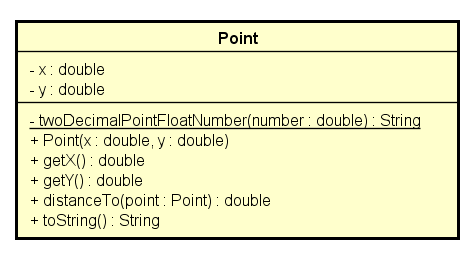
\includegraphics[scale=0.6]{class_point}
	\caption[Diagram kelas \textit{Point}]{Diagram kelas \textit{Point}}
	\label{fig:class_point}
\end{figure}

Kelas ini merepresentasikan titik koordinat 2D. Diagram kelas \textit{Point} dapat dilihat pada gambar~\ref{fig:class_point}. Berikut ini merupakan atribut-atribut yang terdapat pada kelas \textit{Point}:
\begin{itemize}
	\item \textbf{\textit{x} \(\rightarrow\) \textit{double}}\\
	Atribut ini berguna untuk menampung nilai titik pada sumbu x.
	\item \textbf{\textit{y} \(\rightarrow\) \textit{double}}\\
	Atribut ini berguna untuk menampung nilai titik pada sumbu y.
\end{itemize}
Berikut ini merupakan fungsi-fungsi yang terdapat pada kelas \textit{Point}:
\begin{itemize}
	\item \textbf{\textit{twoDecimalPointFloatNumber}(\textit{number} \(\rightarrow\) \textit{double}) \(\rightarrow\) \textit{String}}\\
	Fungsi ini merupakan fungsi statis yang berguna untuk mengubah bilangan \textit{number} ke dalam bentuk \textit{String} dengan maksimal bilangan di belakang koma berjumlah 2 buah.
	\item \textbf{\textit{distanceTo}(\textit{point} \(\rightarrow\) \textit{Point}) \(\rightarrow\) \textit{double}}\\
	Fungsi ini berguna untuk mendapatkan jarak antara titik objek ini dengan titik objek \textit{point}.
\end{itemize}

\subsection{Kelas \textit{CameraSpecification}}
\begin{figure}[H]
	\centering  
	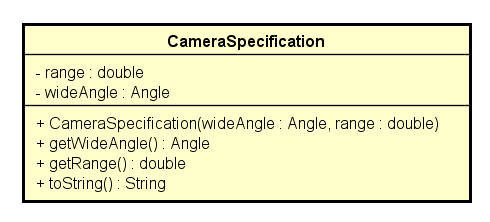
\includegraphics[scale=0.6]{class_camera_specification}
	\caption[Diagram kelas \textit{CameraSpecification}]{Diagram kelas \textit{CameraSpecification}}
	\label{fig:class_camera_specification}
\end{figure}

Kelas ini merepresentasikan spesifikasi kamera CCTV yang terdiri dari jarak pandang dan besar sudut pandang. Diagram kelas \textit{CameraSpecification} dapat dilihat pada gambar~\ref{fig:class_camera_specification}. Berikut ini merupakan atribut-atribut yang terdapat pada kelas \textit{CameraSpecification}:
\begin{itemize}
	\item \textbf{\textit{range} \(\rightarrow\) \textit{double}}\\
	Atribut ini berguna untuk menampung jarak pandang kamera CCTV.
	\item \textbf{\textit{wideAngle} \(\rightarrow\) \textit{Angle}}\\
	Atribut ini berguna untuk menampung besar sudut pandang kamera CCTV.
\end{itemize}

\subsection{Kelas \textit{CameraPlacement}}
\begin{figure}[H]
	\centering  
	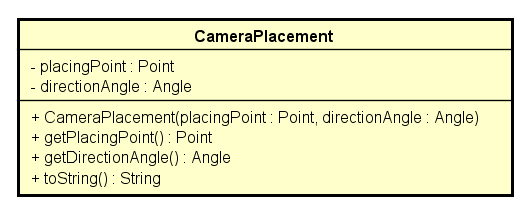
\includegraphics[scale=0.6]{class_camera_placement}
	\caption[Diagram kelas \textit{CameraPlacement}]{Diagram kelas \textit{CameraPlacement}}
	\label{fig:class_camera_placement}
\end{figure}

Kelas ini merepresentasikan penempatan kamera CCTV yang terdiri dari posisi dan sudut arah pandang. Diagram kelas \textit{CameraPlacement} dapat dilihat pada gambar~\ref{fig:class_camera_placement}. Berikut ini merupakan atribut-atribut yang terdapat pada kelas \textit{CameraPlacement}:
\begin{itemize}
	\item \textbf{\textit{placingPoint} \(\rightarrow\) \textit{Point}}\\
	Atribut ini berguna untuk menampung posisi penempatan kamera CCTV.
	\item \textbf{\textit{directionAngle} \(\rightarrow\) \textit{Angle}}\\
	Atribut ini berguna untuk menampung sudut arah pandang kamera CCTV.
\end{itemize}

\subsection{Kelas \textit{Dimension}}
\begin{figure}[H]
	\centering  
	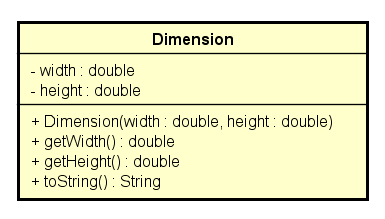
\includegraphics[scale=0.6]{class_dimension}
	\caption[Diagram kelas \textit{Dimension}]{Diagram kelas \textit{Dimension}}
	\label{fig:class_dimension}
\end{figure}

Kelas ini merepresentasikan dimensi yang terdiri dari panjang dan lebar. Diagram kelas \textit{Dimension} dapat dilihat pada gambar~\ref{fig:class_dimension}. Berikut ini merupakan atribut-atribut yang terdapat pada kelas \textit{Dimension}:
\begin{itemize}
	\item \textbf{\textit{width} \(\rightarrow\) \textit{double}}\\
	Atribut ini berguna untuk menampung ukuran lebar.
	\item \textbf{\textit{length} \(\rightarrow\) \textit{double}}\\
	Atribut ini berguna untuk menampung ukuran panjang.
\end{itemize}

\subsection{Kelas \textit{Cell}}
\begin{figure}[H]
	\centering  
	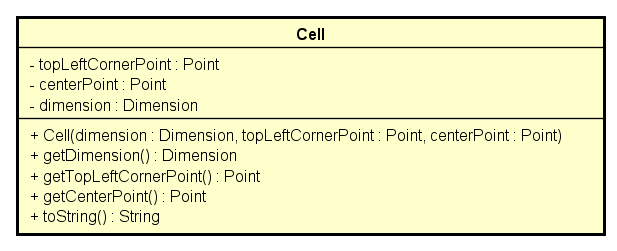
\includegraphics[scale=0.6]{class_cell}
	\caption[Diagram kelas \textit{Cell}]{Diagram kelas \textit{Cell}}
	\label{fig:class_cell}
\end{figure}

Kelas ini merepresentasikan cell. Diagram kelas \textit{Cell} dapat dilihat pada gambar~\ref{fig:class_cell}. Berikut ini merupakan atribut-atribut yang terdapat pada kelas \textit{Cell}:
\begin{itemize}
	\item \textbf{\textit{topLeftCornerPoint} \(\rightarrow\) \textit{Point}}\\
	Atribut ini berguna untuk menampung titik ujung kiri atas cell.
	\item \textbf{\textit{centerPoint} \(\rightarrow\) \textit{Point}}\\
	Atribut ini berguna untuk menampung titik tengah cell.
	\item \textbf{\textit{dimension} \(\rightarrow\) \textit{Dimension}}\\
	Atribut ini berguna untuk menampung dimensi cell.
\end{itemize}

\subsection{Kelas \textit{CellMatrix}}
\begin{figure}[H]
	\centering  
	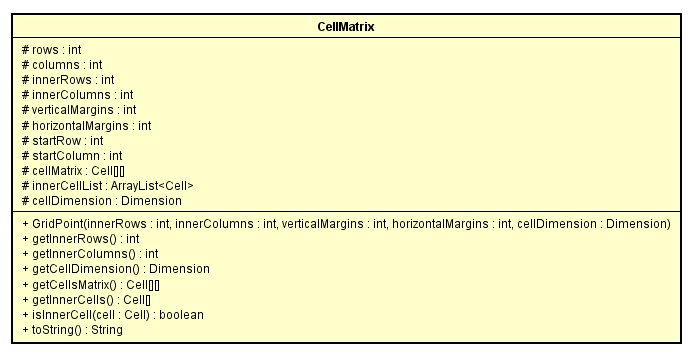
\includegraphics[scale=0.6]{class_cell_matrix}
	\caption[Diagram kelas \textit{CellMatrix}]{Diagram kelas \textit{CellMatrix}}
	\label{fig:class_cell_matrix}
\end{figure}

Kelas ini merepresentasikan matriks \textit{cell} dalam ruangan. Diagram kelas \textit{MatrixCell} dapat dilihat pada gambar~\ref{fig:class_cell_matrix}. Berikut ini merupakan atribut-atribut yang terdapat pada kelas \textit{CellMatrix}:
\begin{itemize}
	\item \textbf{\textit{rows} \(\rightarrow\) \textit{int}}\\
	Atribut ini berguna untuk menampung jumlah baris matriks \textit{cell} secara keseluruhan.
	\item \textbf{\textit{columns} \(\rightarrow\) \textit{int}}\\
	Atribut ini berguna untuk menampung jumlah kolom matriks \textit{cell} secara keseluruhan.
	\item \textbf{\textit{innerRows} \(\rightarrow\) \textit{int}}\\
	Atribut ini berguna untuk menampung jumlah baris matriks \textit{cell} bagian dalam.
	\item \textbf{\textit{innerColumns} \(\rightarrow\) \textit{int}}\\
	Atribut ini berguna untuk menampung jumlah kolom matriks \textit{cell} bagian dalam.
	\item \textbf{\textit{verticalMargins} \(\rightarrow\) \textit{int}}\\
	Atribut ini berguna untuk menampung jumlah margin vertikal matriks \textit{cell}.
	\item \textbf{\textit{horizontalMargins} \(\rightarrow\) \textit{int}}\\
	Atribut ini berguna untuk menampung jumlah margin horizontal matriks \textit{cell}.
	\item \textbf{\textit{startRow} \(\rightarrow\) \textit{int}}\\
	Atribut ini berguna untuk menampung indeks baris pertama matriks \textit{cell} bagian dalam.
	\item \textbf{\textit{startColumn} \(\rightarrow\) \textit{int}}\\
	Atribut ini berguna untuk menampung indeks kolom pertama matriks \textit{cell} bagian dalam.
	\item \textbf{\textit{cellMatrix} \(\rightarrow\) \textit{Cell}[ ][ ]}\\
	Atribut ini berguna untuk menampung matriks \textit{cell} 2 dimensi.
	\item \textbf{\textit{innerCellList} \(\rightarrow\) \textit{ArrayList}<\textit{Cell}>}\\
	Atribut ini berguna untuk menampung seluruh \textit{cell} pada matriks \textit{cell} bagian dalam.
	\item \textbf{\textit{cellDimension} \(\rightarrow\) \textit{Dimension}}\\
	Atribut ini berguna untuk menampung dimensi \textit{cell}.
\end{itemize}

\subsection{Kelas \textit{Room}}
\begin{figure}[H]
	\centering  
	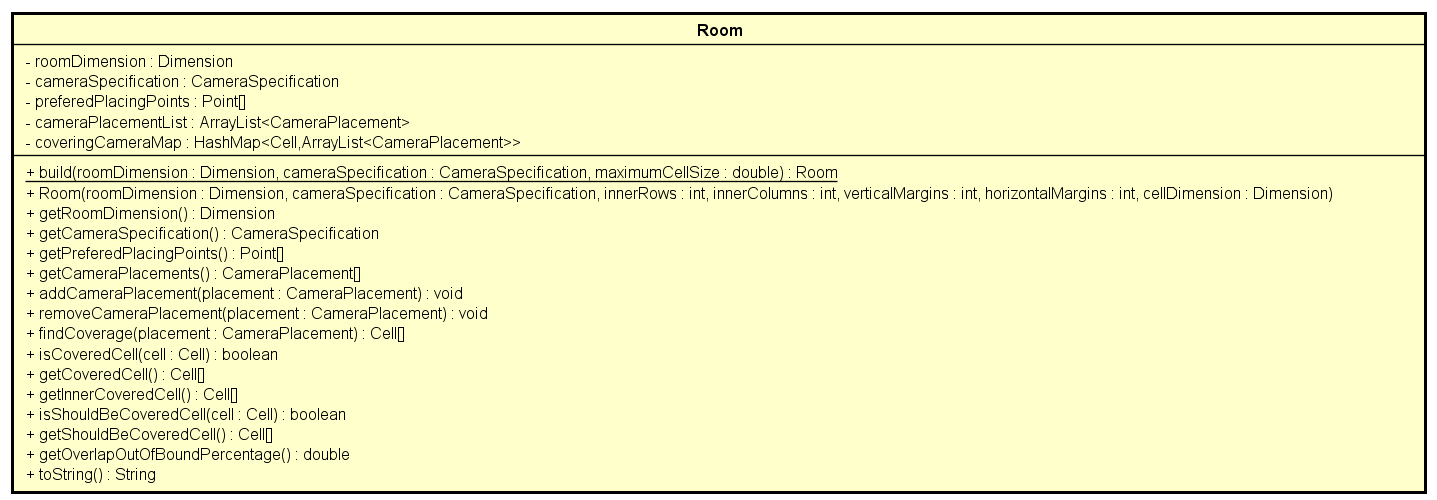
\includegraphics[scale=0.4]{class_room}
	\caption[Diagram kelas \textit{Room}]{Diagram kelas \textit{Room}}
	\label{fig:class_room}
\end{figure}

Kelas ini merepresentasikan ruangan yang dapat diisi oleh kamera-kamera CCTV. Kelas ini merupakan turunan dari kelas \textit{CellMatrix}. Diagram kelas \textit{Room} dapat dilihat pada gambar~\ref{fig:class_room}. Berikut ini merupakan atribut-atribut yang terdapat pada kelas \textit{Room}:
\begin{itemize}
	\item \textbf{\textit{roomDimension} \(\rightarrow\) \textit{Dimension}}\\
	Atribut ini berguna untuk menampung dimensi ruangan.
	\item \textbf{\textit{cameraSpecification} \(\rightarrow\) \textit{CameraSpecification}}\\
	Atribut ini berguna untuk menampung spesifikasi dari kamera CCTV yang akan ditempatkan dalam ruangan.
	\item \textbf{\textit{preferedPlacingPoints} \(\rightarrow\) \textit{Point}[ ]}\\
	Atribut ini berguna untuk menampung posisi-posisi yang dapat ditempati oleh kamera CCTV.
	\item \textbf{\textit{cameraPlacementList} \(\rightarrow\) \textit{ArrayList}<\textit{CameraPlacement}>}\\
	Atribut ini berguna untuk menampung daftar penempatan kamera CCTV.
	\item \textbf{\textit{coveringCameraMap} \(\rightarrow\) \textit{HashMap}<\textit{Cell}, \textit{ArrayList}{<\textit{CameraPlacement}>}>}\\
	Atribut ini berguna untuk menampung pemetaan \textit{cell} dengan penempatan kamera CCTV yang dapat mencakup \textit{cell} tersebut.
\end{itemize}
Berikut ini merupakan fungsi-fungsi yang terdapat pada kelas \textit{Room}:
\begin{itemize}
	\item \textbf{\textit{build}(\textit{roomDimension} \(\rightarrow\) \textit{Dimension}, \textit{cameraSpecification} \(\rightarrow\) \textit{CameraSpecification}, \textit{maximumCellSize} \(\rightarrow\) \textit{double}) \(\rightarrow\) \textit{Room}}\\
	Fungsi ini merupakan fungsi statis yang berguna untuk membuat objek \textit{Room} yang dimana jumlah baris, jumlah kolom, jumlah margin vertikal, jumlah margin horizontal, dan ukuran cell akan ditentukan berdasarkan ukuran ruangan \textit{roomDimension}, spesifikasi kamera \textit{cameraSpecification}, dan ukuran terbesar cell \textit{maximumCellSize}.
	\item \textbf{\textit{addCameraPlacement}(\textit{placement} \(\rightarrow\) \textit{CameraPlacement}) \(\rightarrow\) \textit{void}}\\
	Fungsi ini berguna untuk menambahkan penempatan kamera CCTV ke dalam daftar penempatan kamera CCTV dan memperbaharui pemetaan cell pada atribut \textit{coveringCameraMap}.
	\item \textbf{\textit{removeCameraPlacement}(\textit{placement} \(\rightarrow\) \textit{CameraPlacement}) \(\rightarrow\) \textit{void}}\\
	Fungsi ini berguna untuk membuang penempatan kamera CCTV dari daftar penempatan kamera CCTV dan memperbaharui pemetaan cell pada atribut \textit{coveringCameraMap}.
	\item \textbf{\textit{findCoverage}(\textit{placement} \(\rightarrow\) \textit{CameraPlacement}) \(\rightarrow\) \textit{Cell}[ ]}\\
	Fungsi ini berguna untuk mendapatkan \textit{cell} yang tercakup oleh penempatan kamera CCTV \textit{placement}.
	\item \textbf{\textit{isCoveredCell}(\textit{cell} \(\rightarrow\) \textit{Cell}) \(\rightarrow\) \textit{boolean}}\\
	Fungsi ini berguna untuk mengetahui apakah \textit{cell} telah tercakup oleh setidaknya 1 penempatan kamera CCTV.
	\item \textbf{\textit{getCoveredCell}() \(\rightarrow\) \textit{Cell}[ ]}\\
	Fungsi ini berguna untuk mendapatkan \textit{cell} yang telah tercakup oleh setidaknya 1 penempatan kamera CCTV.
	\item \textbf{\textit{getInnerCoveredCell}() \(\rightarrow\) \textit{Cell}[ ]}\\
	Fungsi ini berguna untuk mendapatkan \textit{cell} yang berada pada matriks \textit{cell} bagian dalam yang telah tercakup oleh setidaknya 1 penempatan kamera CCTV.
	\item \textbf{\textit{isShouldBeCoveredCell}(\textit{cell} \(\rightarrow\) \textit{Cell}) \(\rightarrow\) \textit{boolean}}\\
	Fungsi ini berguna untuk mengetahui apakah \textit{cell} berada pada matriks \textit{cell} bagian dalam dan belum tercakup oleh setidaknya 1 penempatan kamera CCTV.
	\item \textbf{\textit{getShouldBeCoveredCell}() \(\rightarrow\) \textit{Cell}[ ]}\\
	Fungsi ini berguna untuk mendapatkan \textit{cell} yang berada pada matriks \textit{cell} bagian dalam dan belum tercakup oleh setidaknya 1 penempatan kamera CCTV.
	\item \textbf{\textit{getOverlapAndOutOfBoundPercentage}() \(\rightarrow\) \textit{double}}\\
	Fungsi ini berguna untuk mendapatkan persentase \textit{overlap} dan \textit{out of bound}.
\end{itemize}

\subsection{Kelas \textit{MinimumCameraPlacementSolver}}
\begin{figure}[H]
	\centering  
	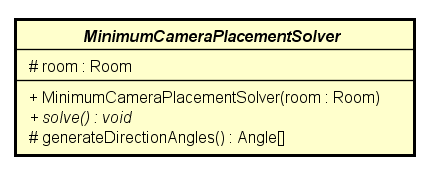
\includegraphics[scale=0.6]{class_minimum_camera_placement_solver}
	\caption[Diagram kelas \textit{MinimumCameraPlacementSolver}]{Diagram kelas \textit{MinimumCameraPlacementSolver}}
	\label{fig:class_minimum_camera_placement_solver}
\end{figure}

Kelas ini merepresentasikan pemecah masalah penempatan kamera CCTV dalam ruangan yang berjumlah minimum yang dapat mencakup seluruh isi ruangan. Kelas ini merupakan kelas abstrak. Diagram kelas \textit{MinimumCameraPlacementSolver} dapat dilihat pada gambar~\ref{fig:class_minimum_camera_placement_solver}. Berikut ini merupakan atribut-atribut yang terdapat pada kelas \textit{MinimumCameraPlacementSolver}:
\begin{itemize}
	\item \textbf{\textit{room} \(\rightarrow\) \textit{Room}}\\
	Atribut ini berguna untuk menampung ruangan yang di mana masalah penempatan kamera CCTV-nya akan diselesaikan.
	\item \textbf{\textit{possibleOrientation} \(\rightarrow\) \textit{int}}\\
	Atribut ini berguna untuk menampung jumlah kemungkinan sudut arah pandang kamera CCTV.
\end{itemize}
Berikut ini merupakan fungsi-fungsi yang terdapat pada kelas \textit{Room}:
\begin{itemize}
	\item \textbf{\textit{solve}() \(\rightarrow\) \textit{void}}\\
	Fungsi ini merupakan fungsi abstrak yang bertujuan untuk menyelesaikan masalah penempatan kamera CCTV dalam ruangan yang berjumlah minimum yang dapat mencakup sekuruh isi ruangan.
	\item \textbf{\textit{generateDirectionAngles}() \(\rightarrow\) \textit{Angle}[ ]}\\
	Fungsi ini berguna untuk menghasilkan sudut-sudut arah pandang berdasarkan jumlah kemungkinan sudut arah pandang \textit{possibleOrientation}.
\end{itemize}

\subsection{Kelas \textit{MinimumCameraPlacementSolverBalasAdditive}}
\begin{figure}[H]
	\centering  
	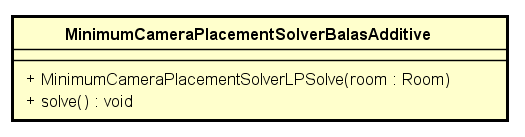
\includegraphics[scale=0.6]{class_minimum_camera_placement_solver_balas_additive}
	\caption[Diagram kelas \textit{MinimumCameraPlacementSolverBalasAdditive}]{Diagram kelas \textit{MinimumCameraPlacementSolverBalasAdditive}}
	\label{fig:class_minimum_camera_placement_solver_balas_additive}
\end{figure}

Kelas ini merepresentasikan pemecah masalah penempatan kamera CCTV dalam ruangan yang berjumlah minimum yang dapat mencakup seluruh isi ruangan dengan menggunakan algoritma \textit{Balas's additive}~(\ref{balas_additive}). Kelas ini merupakan turunan dari kelas MinimumCameraPlacementSolver. Diagram kelas \textit{MinimumCameraPlacementSolverBalasAdditive} dapat dilihat pada gambar~\ref{fig:class_minimum_camera_placement_solver_balas_additive}. Berikut ini merupakan fungsi-fungsi yang terdapat pada kelas \textit{MinimumCameraPlacementSolverBalasAdditive}:
\begin{itemize}
	\item \textbf{\textit{solve}() \(\rightarrow\) \textit{void}}\\
	Fungsi ini berguna untuk menyelesaikan masalah penempatan kamera CCTV dalam ruangan yang berjumlah minimum yang dapat mencakup seluruh isi ruangan menggunakan algoritma \textit{Balas's additive}.
\end{itemize}

\subsection{Kelas \textit{Variable}}
\begin{figure}[H]
	\centering  
	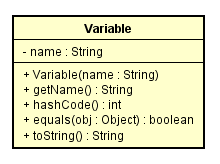
\includegraphics[scale=0.6]{class_variable}
	\caption[Diagram kelas \textit{Variable}]{Diagram kelas \textit{Variable}}
	\label{fig:class_variable}
\end{figure}

Kelas ini merepresentasikan variabel. Diagram kelas \textit{Variable} dapat dilihat pada gambar~\ref{fig:class_variable}. Berikut ini merupakan atribut-atribut yang terdapat pada kelas \textit{Variable}:
\begin{itemize}
	\item \textbf{\textit{name} $\rightarrow$ \textit{String}}\\
	Atribut ini berguna untuk menampung nama variabel.
\end{itemize}

\subsection{Kelas \textit{BIPFunction}}
\begin{figure}[H]
	\centering  
	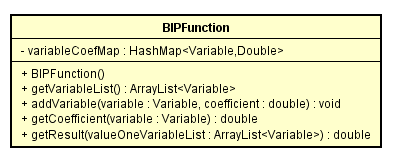
\includegraphics[scale=0.6]{class_bip_function}
	\caption[Diagram kelas \textit{BIPFunction}]{Diagram kelas \textit{BIPFunction}}
	\label{fig:class_bip_function}
\end{figure}

Kelas ini merepresentasikan persamaan yang terdiri dari variabel biner. Diagram kelas \textit{BIPFunction} dapat dilihat pada gambar~\ref{fig:class_bip_function}. Berikut ini merupakan atribut-atribut yang terdapat pada kelas \textit{BIPFunction}:
\begin{itemize}
	\item \textbf{\textit{variableCoefMap} $\rightarrow$ \textit{HashMap}<\textit{Variable}, \textit{Double}>}\\
	Atribut ini berguna untuk menampung koefisien dari setiap variabel.
\end{itemize}
Berikut ini merupakan fungsi-fungsi yang terdapat pada kelas \textit{BIPFunction}:
\begin{itemize}
	\item \textbf{\textit{getVariableList}() $\rightarrow$ \textit{ArrayList}<\textit{Variable}>}\\
	Fungsi ini berguna untuk mendapatkan variabel yang terdapat dalam persamaan.
	\item \textbf{\textit{addVariable}(\textit{variable} $\rightarrow$ \textit{Variable}, \textit{coefficient} $\rightarrow$ \textit{double}) $\rightarrow$ \textit{void}}\\
	Fungsi ini berguna untuk menambahkan variabel beserta koefisiennya ke dalam persamaan.
	\item \textbf{\textit{getCoefficient}(\textit{variable} $\rightarrow$ \textit{Variable}) $\rightarrow$ \textit{double}}\\
	Fungsi ini berguna untuk mendapatkan koefisien dari variabel \textit{variable}.
	\item \textbf{\textit{getResult}(\textit{valueOneVariableList} $\rightarrow$ \textit{ArrayList}<\textit{Variable}>) $\rightarrow$ \textit{double}}\\
	Fungsi ini berguna untuk mendapatkan hasil persamaan berdasarkan daftar variabel yang bernilai 1.
\end{itemize}

\subsection{Kelas \textit{BIPConstraint}}
\begin{figure}[H]
	\centering  
	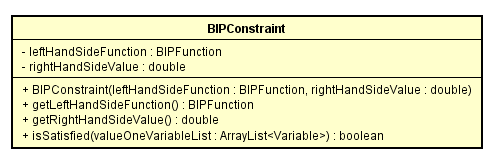
\includegraphics[scale=0.6]{class_bip_constraint}
	\caption[Diagram kelas \textit{BIPConstraint}]{Diagram kelas \textit{BIPConstraint}}
	\label{fig:class_bip_constraint}
\end{figure}
Kelas ini merepresentasikan batasan dalam masalah \textit{binary integer programming}. Diagram kelas \textit{BIPConstraint} dapat dilihat pada gambar~\ref{fig:class_bip_constraint}. Berikut ini merupakan atribut-atribut yang terdapat pada kelas \textit{BIPConstraint}:
\begin{itemize}
	\item \textbf{\textit{leftHandSideFunction} $\rightarrow$ \textit{BIPFunction}}\\
	Atribut ini berguna untuk menampung persamaan pada ruas kiri batasan.
	\item \textbf{\textit{rightHandSideValue} $\rightarrow$ \textit{double}}\\
	Atribut ini berguna untuk menampung nilai pada ruas kanan batasan.
\end{itemize}
Berikut ini merupakan fungsi-fungsi yang terdapat pada kelas \textit{BIPConstraint}:
\begin{itemize}
	\item \textbf{\textit{isSatisfied}(\textit{valueOneVariableList} $\rightarrow$ \textit{ArrayList}<\textit{Variable}>) $\rightarrow$ \textit{boolean}}\\
	Fungsi ini berguna untuk mengetahui apakah batasan dapat dipenuhi berdasarkan daftar variabel yang bernilai 1.
\end{itemize}

\subsection{Kelas \textit{BIPProblem}}
\begin{figure}[H]
	\centering  
	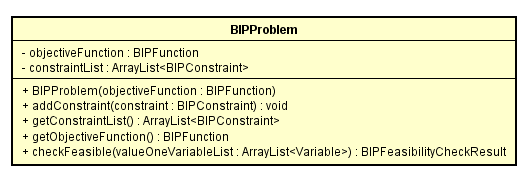
\includegraphics[scale=0.6]{class_bip_problem}
	\caption[Diagram kelas \textit{BIPProblem}]{Diagram kelas \textit{BIPProblem}}
	\label{fig:class_bip_problem}
\end{figure}
Kelas ini merepresentasikan model masalah \textit{binary integer programming}. Diagram kelas \textit{BIPProblem} dapat dilihat pada gambar~\ref{fig:class_bip_problem}. Berikut ini merupakan atribut-atribut yang terdapat pada kelas \textit{BIPProblem}:
\begin{itemize}
	\item \textbf{\textit{objectiveFunction} $\rightarrow$ \textit{BIPFunction}}\\
	Atribut ini berguna untuk menampung persaman fungsi tujuan.
	\item \textbf{\textit{constraintList} $\rightarrow$ \textit{ArrayList}<\textit{BIPConstraint}>}\\
	Atribut ini berguna untuk menampung batasan-batasan.
\end{itemize}
Berikut ini merupakan fungsi-fungsi yang terdapat pada kelas \textit{BIPProblem}:
\begin{itemize}
	\item \textbf{\textit{addConstraint}(\textit{constraint} $\rightarrow$ \textit{BIPConstraint}) $\rightarrow$ \textit{void}}\\
	Fungsi ini berguna untuk menambahkan batasan pada model masalah \textit{binary integer programming}.
	\item \textbf{\textit{checkFeasible}(\textit{valueOneVariableList} $\rightarrow$ \textit{ArrayList}<\textit{Variable}>) $\rightarrow$ \textit{BIPFeasibilityCheckResult}}\\
	Fungsi ini berguna untuk mengembalikan hasil pengecekan solusi \textit{feasible} berdasarkan daftar variabel bernilai 1.
\end{itemize}

\subsection{Kelas \textit{BIPFeasibilityCheckResult}}
\begin{figure}[H]
	\centering  
	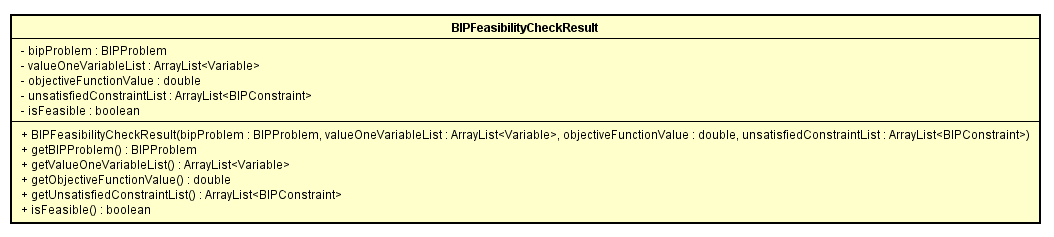
\includegraphics[scale=0.6]{class_bip_feasibility_check_result}
	\caption[Diagram kelas \textit{BIPFeasibilityCheckResult}]{Diagram kelas \textit{BIPFeasibilityCheckResult}}
	\label{fig:class_bip_feasibility_check_result}
\end{figure}
Kelas ini merepresentasikan hasil pengecekan solusi \textit{feasible} pada masalah \textit{binary integer programming}. Diagram kelas \textit{BIPFeasibilityCheckResult} dapat dilihat pada gambar~\ref{fig:class_bip_feasibility_check_result}. Berikut ini merupakan atribut-atribut yang terdapat pada kelas \textit{BIPFeasibilityCheckResult}:
\begin{itemize}
	\item \textbf{\textit{blpProblem} $\rightarrow$ \textit{BLPProblem}}\\
	Atribut ini berguna untuk menampung model masalah \textit{binary integer programming}.
	\item \textbf{\textit{valueOneVariableList} $\rightarrow$ \textit{ArrayList}<\textit{\textit{Variable}}>}\\
	Atribut ini berguna untuk menampung solusi berupa daftar variabel yang bernilai 1.
	\item \textbf{\textit{objectiveFunctionValue} $\rightarrow$ \textit{double}}\\
	Atribut ini berfungsi untuk menampung nilai hasil fungsi tujuan.
	\item \textbf{\textit{unsatisfiedConstraintList} $\rightarrow$ \textit{ArrayList}<\textit{BIPConstraint}>}\\
	Atribut ini berfungsi untuk menampung batasan-batasan yang tidak dipenuhi.
	\item \textbf{\textit{isFeasible} $\rightarrow$ \textit{boolean}}\\
	Atribut ini berfungsi untuk menampung apakah solusi bersifat \textit{feasible}.
\end{itemize}

\subsection{Kelas \textit{Node}}
\begin{figure}[H]
	\centering  
	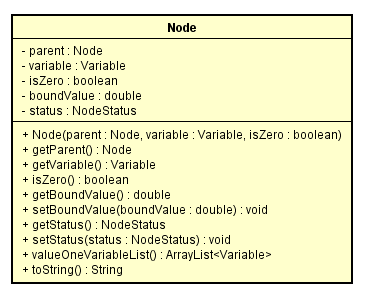
\includegraphics[scale=0.6]{class_node}
	\caption[Diagram kelas \textit{Node}]{Diagram kelas \textit{Node}}
	\label{fig:class_node}
\end{figure}
Kelas ini merepresentasikan \textit{node} yang digunakan dalam algoritma \textit{Balas's additive}. Diagram kelas \textit{Node} dapat dilihat pada gambar~\ref{fig:class_node}. Berikut ini merupakan atribut-atribut yang terdapat pada kelas \textit{Node}:
\begin{itemize}
	\item \textbf{\textit{parent} $\rightarrow$ \textit{Node}}\\
	Atribut ini berguna untuk menampung orang tua dari \textit{node} ini.
	\item \textbf{\textit{variable} $\rightarrow$ \textit{Variable}}\\
	Atribut ini berguna untuk menampung variabel yang dituju oleh \textit{node} ini.
	\item \textbf{\textit{isZero} $\rightarrow$ \textit{boolean}}\\
	Atribut ini berguna untuk menampung apakah variabel pada \textit{node} ini bernilai 1.
	\item \textbf{\textit{boundValue} $\rightarrow$ \textit{double}}\\
	Atribut ini berguna untuk menampung nilai \textit{bound} dari \textit{node} ini.
	\item \textbf{\textit{status} $\rightarrow$ \textit{NodeStatus}}\\
	Atribut ini berguna untuk menampung status dari \textit{node} ini.
\end{itemize}
Berikut ini merupakan fungsi-fungsi yang terdapat pada kelas \textit{Node}:
\begin{itemize}
	\item \textbf{\textit{valueOneVariableList}() $\rightarrow$ \textit{ArrayList}<\textit{Variable}>}\\
	Fungsi ini berguna untuk menghasilkan daftar variabel bernilai 1 yang dimulai dari \textit{node} ini hingga \textit{root node}.
\end{itemize}

\subsection{Kelas \textit{NodeStatus}}
\begin{figure}[H]
	\centering  
	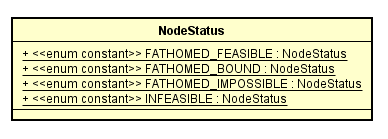
\includegraphics[scale=0.6]{enum_node_status}
	\caption[Diagram kelas \textit{NodeStatus}]{Diagram kelas \textit{NodeStatus}}
	\label{fig:enum_node_status}
\end{figure}
Kelas ini merepresentasikan status yang dapat dimiliki oleh \textit{node}. Diagram kelas \textit{NodeStatus} dapat dilihat pada gambar~\ref{fig:enum_node_status}. Berikut ini merupakan pilihan-pilihan status yang terdapat pada kelas \textit{NodeStatus}:
\begin{itemize}
	\item \textbf{\textit{FATHOMED\_FEASIBLE} $\rightarrow$ \textit{NodeStatus}}\\
	Pilihan ini menyatakan status \textit{fathomed} dengan alasan solusi \textit{feasible}.
	\item \textbf{\textit{FATHOMED\_BOUND} $\rightarrow$ \textit{NodeStatus}}\\
	Pilihan ini menyatakan status \textit{fathomed} dengan alasan nilai \textit{bound} yang lebih buruk daripada solusi \textit{incumbent}.
	\item \textbf{\textit{FATHOMED\_IMPOSSIBLE} $\rightarrow$ \textit{NodeStatus}}\\
	Pilihan ini menyatakan status \textit{fathomed} dengan alasan \textit{impossible} atau tidak dapat menghasilkan \textit{incumbent}.
	\item \textbf{\textit{INFEASIBLE} $\rightarrow$ \textit{NodeStatus}}\\
	Pilihan ini menyatakan status \textit{infeasible}
\end{itemize}

\subsection{Kelas BalasAdditiveBIPSolver}
\begin{figure}[H]
	\centering  
	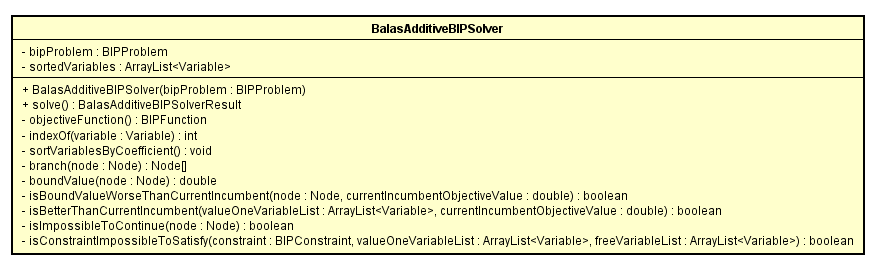
\includegraphics[scale=0.6]{class_balas_additive_bip_solver}
	\caption[Diagram kelas \textit{BalasAdditiveBIPSolver}]{Diagram kelas \textit{BalasAdditiveBIPSolver}}
	\label{fig:class_balas_additive_bip_solver}
\end{figure}
Kelas ini merepresentasikan metode penyelesaian masalah \textit{binary integer programming} menggunakan algoritma \textit{Balas's additive}. Diagram kelas \textit{BalasAdditiveBIPSolver} dapat dilihat pada gambar~\ref{fig:class_balas_additive_bip_solver}. Berikut ini merupakan atribut-atribut yang terdapat pada kelas \textit{BalasAdditiveBIPSolver}:
\begin{itemize}
	\item \textbf{\textit{bipProblem} $\rightarrow$ \textit{BIPProblem}}\\
	Atribut ini berguna untuk menampung model masalah \textit{binary integer programming} yang akan diselesaikan.
	\item \textbf{\textit{sortedVariables} $\rightarrow$ \textit{ArrayList}<\textit{Variable}>}\\
	Atribut ini berfungsi untuk menampung variabel biner yang telah diurut menaik berdasarkan koefisiennya.
\end{itemize}
Berikut ini merupakan fungsi-fungsi yang terdapat pada kelas \textit{BalasAdditiveBIPSolver}:
\begin{itemize}
	\item \textbf{\textit{solve}() $\rightarrow$ \textit{BalasAdditiveBIPSolverResult}}\\
	Fungsi ini berguna untuk mendapatkan solusi masalah \textit{bipProblem} menggunakan algoritma \textit{Balas's additive}.
	\item \textbf{\textit{objectiveFunction}() $\rightarrow$ \textit{BIPFunction}}\\
	Fungsi ini berguna untuk mendapatkan fungsi tujuan dari masalah \textit{bipProblem}.
	\item \textbf{\textit{indexOf}(\textit{variable} $\rightarrow$ \textit{Variable}) $\rightarrow$ \textit{int}}\\
	Fungsi ini berguna untuk mendapatkan indeks \textit{variable} dalam daftar variabel yang telah terurut.
	\item \textbf{\textbf{sortVariablesByCoefficient}() $\rightarrow$ \textbf{void}}\\
	Fungsi ini berguna untuk mengurutkan variabel secara menaik berdasarkan koefisiennya.
	\item \textbf{\textit{branch}(\textit{node} $\rightarrow$ \textit{Node}) $\rightarrow$ \textit{Node} [ ]}\\
	Fungsi ini berguna untuk membuat cabang \textit{node}-0 dan \textit{node}-1 dari \textit{node}.
	\item \textbf{\textit{boundValue}(\textit{node} $\rightarrow$ \textit{Node}) $\rightarrow$ \textit{double}}\\
	Fungsi ini berguna untuk menghitung nilai \textit{bound} dari \textit{node}.
	\item \textbf{\textit{isBoundValueWorseThanCurrentIncumbent}(\textit{node} $\rightarrow$ \textit{Node}, \textit{currentIncumbentObjectiveValue} $\rightarrow$ \textit{double}) $\rightarrow$ \textit{boolean}}\\
	Fungsi ini berguna untuk mengetahui apakah nilai \textit{bound} pada \textit{node} lebih buruk daripada nilai solusi \textit{incumbent}.
	\item \textbf{\textit{isBetterThanCurrentIncumbent}(\textit{valueOneVariableList} $\rightarrow$ \textit{ArrayList}<\textit{Variable}>, \textit{currentIncumbentObjectiveValue} $\rightarrow$ \textit{double}) $\rightarrow$ \textit{boolean}}\\
	Fungsi ini berguna untuk mengetahui apakah daftar variabel bernilai 1 dapat menghasilkan solusi yang lebih baik daripada solusi \textit{incumbent}.
	\item \textbf{\textit{isImpossibleToContinue}(\textit{node} $\rightarrow$ \textit{Node}) $\rightarrow$ \textit{boolean}}\\
	Fungsi ini berguna untuk mengetahui apakah \textit{node} tidak mungkin untuk menghasilkan \textit{incumbent}.
	\item \textbf{\textit{isConstraintImpossibleToSatisfy}(\textit{constraint} $\rightarrow$ \textit{BIPConstraint}, \textit{valueOneVariableList} $\rightarrow$ \textit{ArrayList}<\textit{Variable}>, \textit{freeVariableList} $\rightarrow$ \textit{ArrayList}<\textit{Variable}>) $\rightarrow$ \textit{boolean}}\\
	Fungsi ini berguna untuk mengetahui apakah \textit{constraint} dapat dipenuhi berdasarkan daftar variabel bernilai 1 dan daftar variabel bebas.
\end{itemize}

\subsection{Kelas \textit{BalasAdditiveBIPSolverResult}}
\begin{figure}[H]
	\centering  
	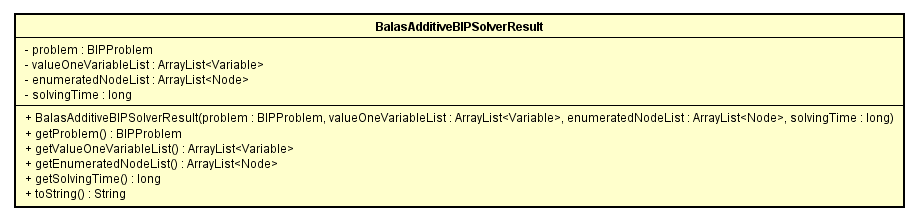
\includegraphics[scale=0.6]{class_balas_additive_bip_solver_result}
	\caption[Diagram kelas \textit{BalasAdditiveBIPSolverResult}]{Diagram kelas \textit{BalasAdditiveBIPSolverResult}}
	\label{fig:class_balas_additive_bip_solver_result}
\end{figure}
Kelas ini merepresentasikan hasil dari penyelesaian masalah \textit{binary integer programming} menggunakan algoritma \textit{Balas's additive}. Diagram kelas \textit{BalasAdditiveBIPSolverResult} dapat dilihat pada gambar~\ref{fig:class_balas_additive_bip_solver_result}. Berikut ini merupakan atribut-atribut yang terdapat pada kelas \textit{BalasAdditiveBIPSolverResult}:
\begin{itemize}
	\item \textbf{\textit{bipProblem} $\rightarrow$ \textit{BIPProblem}}\\
	Atribut ini berguna untuk menampung model masalah \textit{binary integer programming}.
	\item \textbf{\textit{valueOneVariableList} $\rightarrow$ \textit{ArrayList}<\textit{Variable}>}\\
	Atribut ini berguna untuk menampung solusi penyelesaian berupa daftar variabel yang bernilai~1.
	\item \textbf{\textit{enumeratedNodeList} $\rightarrow$ \textit{ArrayList}<\textit{Node}>}\\
	Atribut ini berfungsi untuk menampung daftar \textit{node} yang diperiksa selama melakukan penyelesaian masalah menggunakan algoritma \textit{Balas's additive}.
	\item \textbf{\textit{solvingTime} $\rightarrow$ \textit{long}}\\
	Atribut ini berfungsi untuk menampung waktu yang digunakan dalam menyelesaikan masalah dalam satuan milisekon.
\end{itemize}